\clearpage
\section{Upper and lower modulation traces}
\begin{center}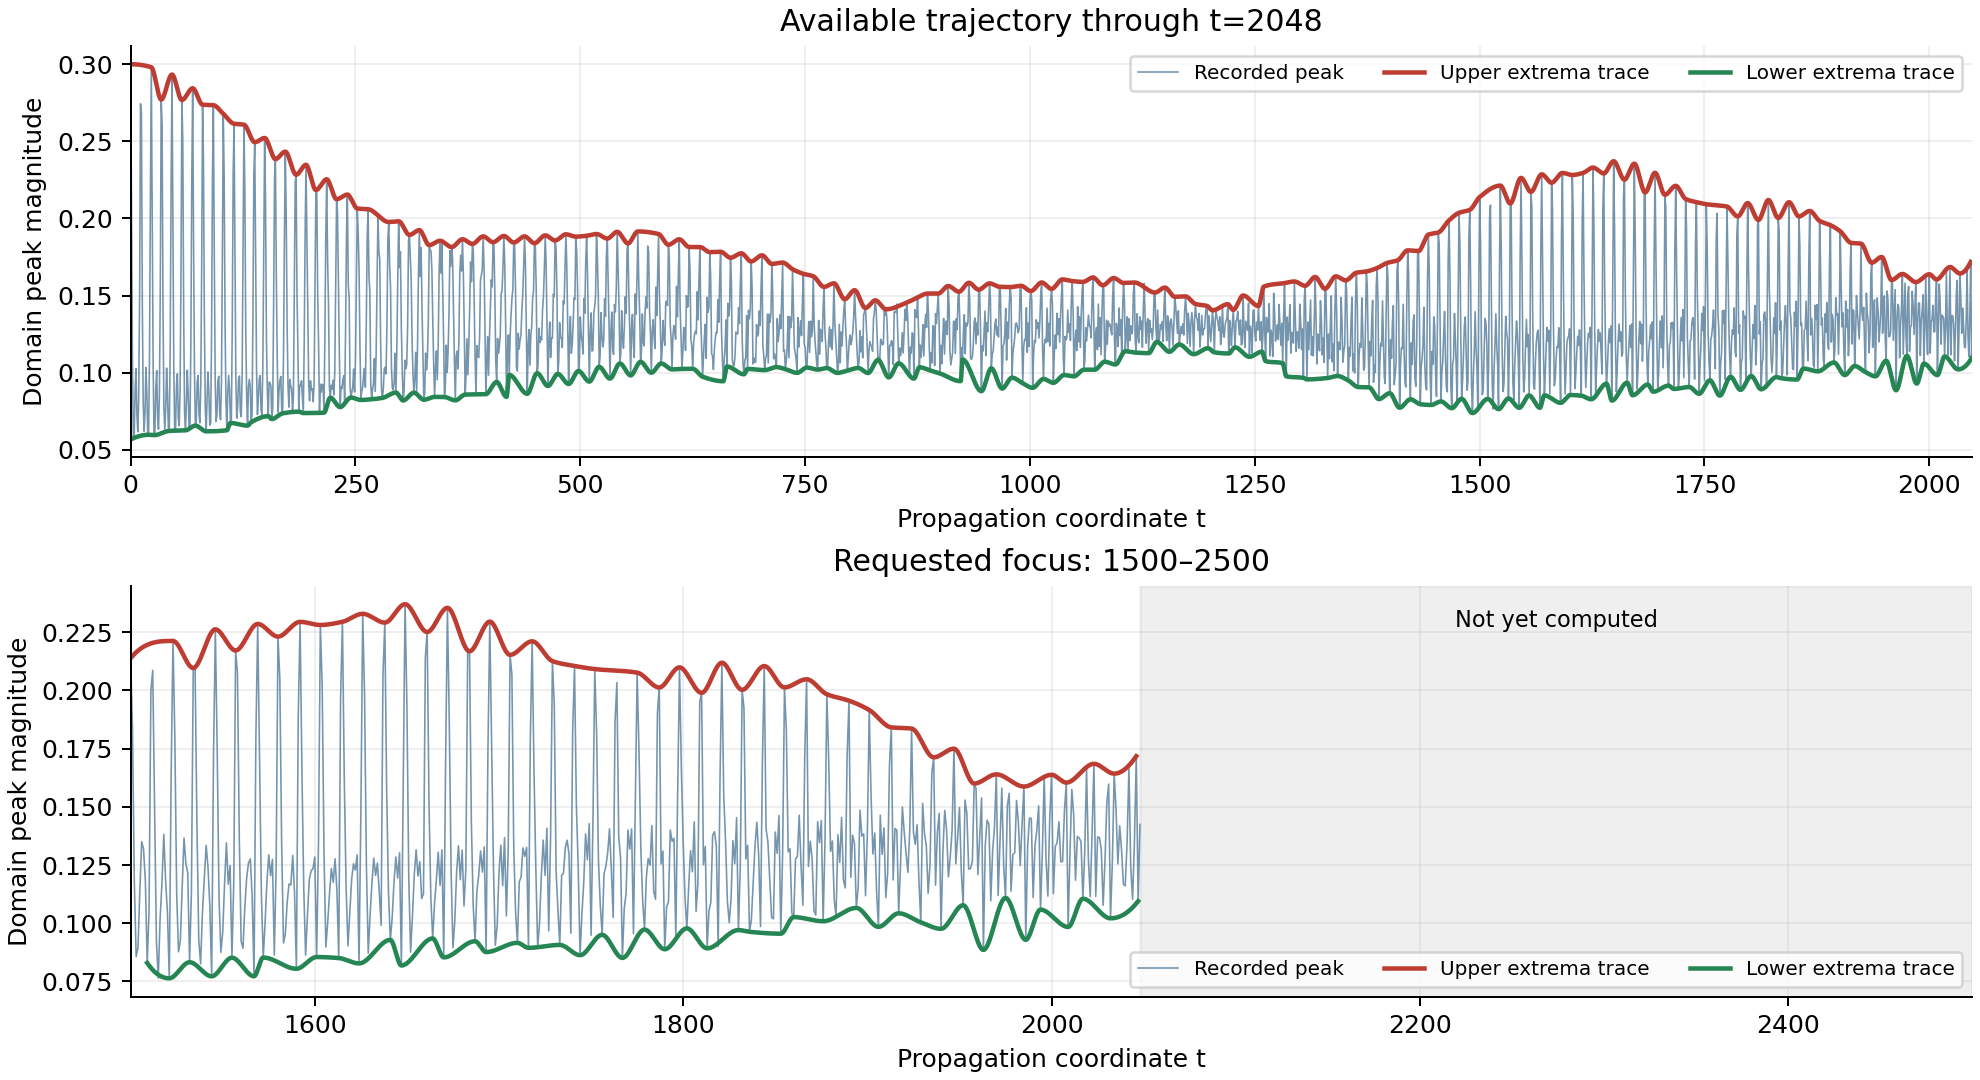
\includegraphics[width=\linewidth]{peak_envelopes.png}\end{center}
\noindent\textbf{Peak envelopes.} Red and green curves trace the maximum and minimum in successive 12-unit intervals using shape-preserving cubic interpolation. This bin length approximates the fitted base oscillation period. These descriptive traces are not guaranteed mathematical bounds; binning and temporal sampling can miss extrema. They do not extrapolate past available observations.

The separation between the traces highlights slow changes in oscillation amplitude. Around $t=1500$--$1750$, the upper peaks rise while the lower trace stays substantially lower. This is consistent with stronger modulation, but does not by itself show that a localized pulse narrows and widens. Spatial width, concentration, and phase are absent from this submitted dataset.

The requested focus is $1500\leq t\leq2500$. The shaded region after $2048$ is deliberately left without data because this fine-step trajectory ends there. The separate coarse preview covers the full focus interval and supplies concentration measures and thousand-point showcases later in this report. Its samples are not spliced into this figure because its grid and time step differ.
